\section{System Overview}

% Overview
Our 3DTI system fuses two distributed scenes into a virtual space in full 3D. The end-to-end delay is 50 ms, i.e., the time interval between a user acts and his remote partner sees. The system consists of inexpensive commercial devices (\$ 7000). The project is open-source [?]. Figure xxx illustrates the pipeline of our system.

%Each side: CPU $400; GPU $700; network card $400; RAM $200; Disk $200; HTC Vive $1200; Realsense $150*3.

\subsection{Hardware and Software Overview}

\subsubsection{Hardware}

At each capture site, we had three depth cameras for capturing, a PC for computing and an HMD for rendering. Realsense D415 (depth cameras) were used to capture a volume of $2m \times 2m \times 2m$. The locating place of each camera and its contribution to 3D mesh are illustrated in Figure xx. Each PC had an Intel i7-7700k CPU and a GTX 1080Ti GPU. HTC Vive was used to present the fused reconstruction of both sides. Ten Gigabit network cards (Intel X520-SR2) were used to connect the two capture sites.

\subsubsection{Software}

OpenCV was used for camera calibration. CUDA was used for image processing and the kernel algorithm. Unity3D was used to implement the high-level application. It fetches live reconstruction from the kernel and renders it in HTC Vive.

\subsection{Calibration}

\subsubsection{Calibration between Cameras}

The \emph{camera calibration module} in OpenCV was used to calibrate the cameras. Each pair of cameras took ten snapshots (1080p color images) of a glass-made flat checkerboard. Then, OpenCV aligned their coordinates ($SD < 1 pixel$).

%[from lwq] To achieve a more accurate calibration, we use 1080p color imagine and a glass-made flat checkerboard moving in common area. Then we use the OpenCV library to detect corners in checkerboard. By analyzing a series of frames, we can align coordinates of two cameras. This process can reduce the standard deviation between two cameras to 1 pixel.

\subsubsection{Calibration between HMD and Cameras}

The HTC Vive was calibrated by setting the original point in its software. We placed the original point of the cameras at the same position by using the checkerboard. Hence, we aligned the HTC Vive and the cameras. This calibration is not necessarily accurate because the users can hardly perceive the error [?]. This step also aligned the coordinates of the two capture sites.

%[from lwq] First we use a certain point on table as original point of our virtual space. We also use a black and white checkerboard to unify the coordinates of two terminal. After doing this we can merge space of two users into virtual one and they share one common table, sitting in each side of it. Then we put the HTC VIVE on the original point and facing certain direction to calibrate the VR glass and virtual world coordinate. 

\subsection{Preprocessing}

\subsubsection{Depth Processing}

The cameras acquired depth images of $640 \times 480$ pixels at 30 FPS. The Realsense D415 is based on binocular disparity. Thus, disparity values (instead of depth values) were used in the processing for accuracy. We applied median filtering, spatial filtering, hole filling and temporary filtering on the depth images.

%We use CUDA to reimplement the depth processing module in RealSense SDK for efficiency. The RealSense acquires depth images with $640 \times 480$ pixel resolution at 30 FPS. RealSense D400-series are based on binocular disparity. It is more accurate to filter depth information in disparity values. We upload origin images in disparity values from CPU to GPU. Then we apply median filtering, spatial filtering, hole filling and temporary filtering on them. Finally, we translate the disparity values into depth images.

\subsubsection{Color Processing}

% We upload the original images in YUV422 format from CPU to GPU. Finally, we translate images into the RGB format in GPU.

The cameras acquired color images of $960 \times 540$ pixels at 30 FPS. We manually adjusted the explosion setting of the RealSense. We used one RGB camera as a reference and warped the other cameras to this reference by white balancing and linear mapping.

\subsubsection{Background Removal}

The system fuses physical worlds in both sides into a virtual scene. It should remove unnecessary background and retain only the shared objects and the individuals. We recorded RGBD images as background in the calibration step. At runtime, we removed pixels that are similar to the background based on thresholds.

\subsection{3D Reconstruction}

[from lwq]We divide the reality space into $256 \times 256 \times 256$ voxels and calculate SDF values using point clouds provided by all the depth cameras parallelly on GPUs. By doing that we can merge these point clouds. When calculating the SDF value, we use a weighted average instead of simple average where  $W_{i} = \frac{1}{Dist}$, considering the error of Realsense Depth Camera is proportional to the distance from the camera to the object. This process can improve the quality of mesh and reduce some noise from hardware. 
    
As we need to merge point clouds from two clients, we need to retain some objects from the other depth camera array. In one of our application, we fuse two chessboards along with half of the chess each side together to implement remote gaming. In this case, we need to retain the chess from both sides. So we run TSDF on each side separately and take the minimum of SDF values to gain the actual surface of the merged mesh. A simple example of this procession is shown in Figure XX.

\begin{figure*}[!htbp]
\centering
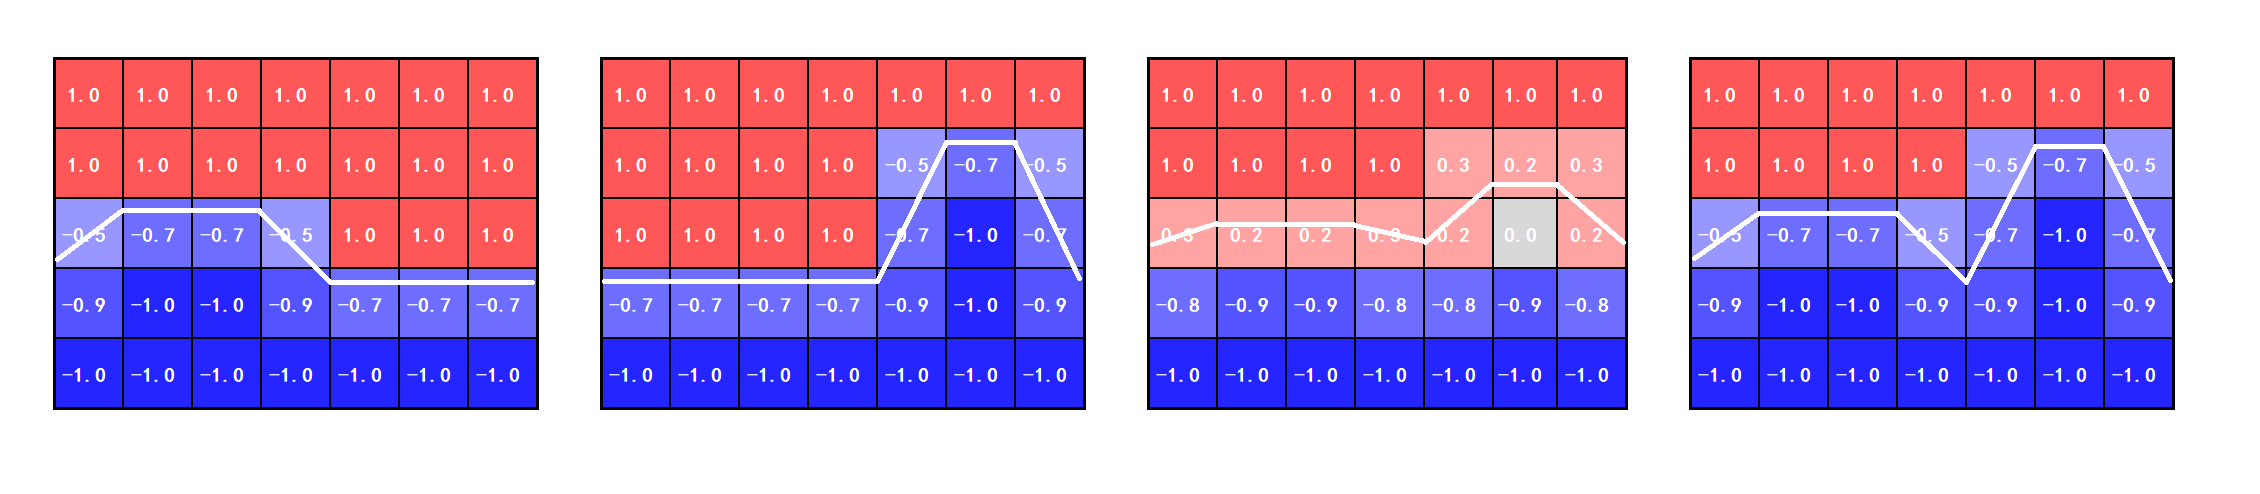
\includegraphics[width=14cm,height=4cm]{figures/figure_tsdf.png}
\setlength{\abovecaptionskip}{-0.5cm}
\caption{Left to right: 1)SDF value from camera 1; 2)Merged SDF value from camera 2; 3)SDF value by simple average; 4)Merged SDF value from our project.}
\label{3}
\end{figure*}
    
Then we use the marching cube to convert the SDF value of each volume to a triangle mesh, which can be done parallelly on GPUs. To fully make use of color images from cameras, we divide one triangle into four triangles by midpoints of each edge. Then we can match color imagine with these triangles for a better texture quality without a large effect on efficiency(Figure YY).

\begin{figure}[H]
\centering
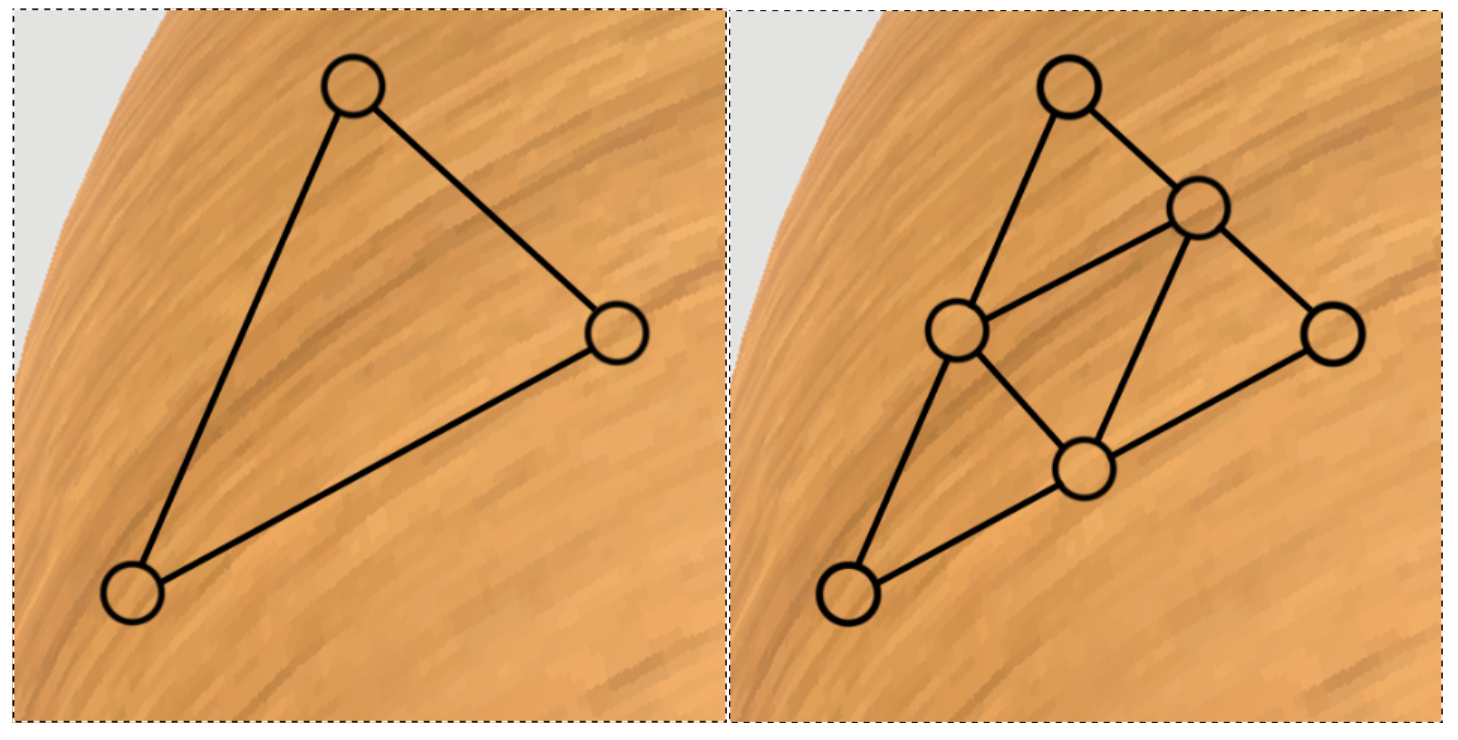
\includegraphics[width=6cm,height=3cm]{figures/figure_mc.png}
\setlength{\abovecaptionskip}{0.5cm}
\caption{Left: Mesh without Supersampling; Right: Mesh witht Supersampling.}
\label{4}
\end{figure}


\subsection{Delay Control}
[from lwq]To gain a more credible result of delay preception in 3DTI, we need to have accurate control over our system. First, we synchronize the depth camera array using Realsense SDK. We set the frame rate of cameras at 30FPS and also regard it as the system clock. After that, we can start our procession when depth cameras obtain new data. The latency of our system is controllable, and it can be minimized to XXXms. Figure XXX shows the pipeline and estimation of the delay of our system when using three depth cameras on each side. To have better control on the delay, we use a buffer to store the data transmitted from the remote client. We can alter the latency by changing the time each set of data remains in the cache.

\begin{figure*}[!htbp]
\centering
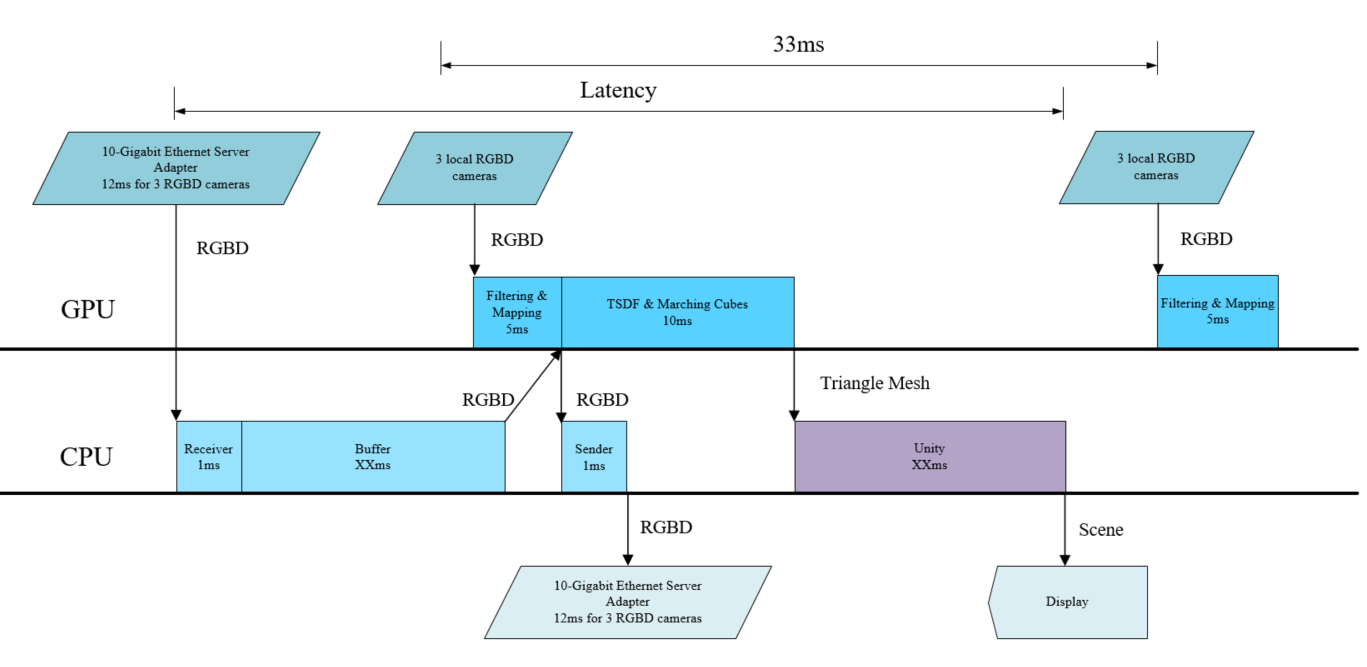
\includegraphics[width=14cm,height=7cm]{figures/figure_pipeline.png}
\setlength{\abovecaptionskip}{0.5cm}
\caption{}
\label{5}
\end{figure*}
